\documentclass[]{scrartcl}

\usepackage{amsmath}
\usepackage{amssymb}
\usepackage[utf8]{inputenc}
\usepackage[T1]{fontenc}
\usepackage{lmodern}
\usepackage{ngerman}
\usepackage{geometry}
\usepackage{graphicx}
\usepackage{wrapfig}
\usepackage{caption}
\usepackage{wasysym}
\usepackage{siunitx}
\usepackage{picinpar}
\usepackage{tikz}
\usepackage{float}

\renewcommand{\figurename}{Abb.}
\usepackage[
	colorlinks=true,
	urlcolor=blue,
	linkcolor=black
]{hyperref}


%Hier Titel und so
\newcommand{\versuchnummer}{V56} 
\newcommand{\versuchname}{Modulation und Demodulation elektrischer Schwingungen} 
\newcommand{\versuchdatum}{Datum} 


\title{Versuch \versuchnummer\\ \versuchname}
\subtitle{Physikalisches Fortgeschrittenenpraktikum}
\author{Robert Rauter und Björn Lindhauer}
\date{\versuchdatum} 
\begin{document}
\begin{titlepage}
{\large \versuchdatum}
\vspace{7cm}
\begin{center}
\textbf{\huge Versuch \versuchnummer:}\\
\vspace{0.5cm}
\textbf{\huge \versuchname}\\
\vspace{0.2cm}
\textbf{ Physikalisches Fortgeschrittenenpraktikum}\\
\vspace{9cm}

{\Large Robert Rauter \ \ \hspace{1.5cm} und \hspace{1.5cm} Björn Lindhauer}\\
{ \url{robert.rauter@tu-dortmund.de} \ \ \hspace{2cm} \url{bjoern.lindhauer@tu-dortmund.de}}
\end{center}
\end{titlepage}
\section{Einleitung}
Unter Modulation wird Veränderung der Amplitude, der Phase oder der Frequenz einer Welle im Rhythmus des Nachrichtensignals verstanden. Sie wird benötigt, um Signale mit elektromagnetische Wellen zu übertragen.\\
Das übertragene Signal muss beim Empfänger anschließend zurück gewonnen werden. Dieser Vorgang wird als Demodulation bezeichnet.\\ Mit der Zeit wurden verschiedene Verfahren mit unterschiedlichen Stärken und Schwächen in der Störsicherheit, im Wirkungsgrad, in der Verzerrungsfreiheit und in der Breite des Frequenzspektrums entwickelt. Diese Verfahren lassen sich in zwei Klassen, den Amplitudenmodulations- und Phasenwinkelmodulation- Verfahren unterteilen.\\
In diesen Versuch sollen Beispiele beider Verfahrensklassen untersucht werden.
\section{Theoretische Grundlagen}
\subsection{Amplitudenmodulation}
Eine Amplitudenmodulation kann durch eine hochfrequente Trägerschwingung $U_{\text{T}}\left(t\right)$ mit niederfrequenten Modulationssignal $U_{\text{M}}\left(t\right)$ erreicht werden.\\
Die zeitliche Entwicklung der Amplituden lassen sich durch
\begin{align}
U_{\text{T}}\left(t\right)=\hat{U}_{\text{T}} \cos \omega_{\text{T}}t  \text{ und }U_{\text{M}}\left(t\right)=\hat{U}_{\text{M}} \cos \omega_{\text{M}}t
\end{align}
darstellen. Dabei sind die $\omega_{i}$ jeweils die Frequenzen und $\hat{U}_{i}$ die Amplituden der Trägerschwingung bzw. der Modulationsschwingung.\\
Daraus folgt für die amplitudenmodulierte Schwingung
\begin{align}
U_3\left(t\right)=\hat{U}_{\text{T}} \left(1+m\cos \omega_{\text{M}}t\right)\cos \omega_{\text{T}}t
\label{eq:amplitudederamplitudenmoduliertenschwingung}
\end{align}
mit den Modulationsgrad genannten Größe
\begin{align}
m=\gamma \hat{U}_{\text{M}} \hspace{0.5cm}\text{.}
\end{align}
Der Modulationsgrad kann nur Werte zwischen 0 und 1 annehmen, sodass die Maxima der modulierten Schwingung zwischen $\hat{U}_{\text{T}}\left(1-m\right)$ und $\hat{U}_{\text{T}}\left(1+m\right)$ liegen, wie in Abbildung 
\ref{fig:zeitabhaengigkeit_momentanspannung} anschaulich dargestellt.
Die Gleichung \ref{eq:amplitudederamplitudenmoduliertenschwingung} lässt sich durch trigonometrischer Beziehungen in die Form
\begin{align}
U_3\left(t\right)=\hat{U}_{\text{T}}\left(\cos \omega_{\text{T}}t+ \frac{m}{2}\cos \left( \omega_{\text{T}}+\omega_{\text{M}}\right)t +\frac{m}{2}\cos \left( \omega_{\text{T}}-\omega_{\text{M}}\right)t  \right) 
\label{eq:amplitudederamplitudenmoduliertenschwingungbesser}
\end{align}
überführen, anhand jener das Frequenzspektrum einfach abgelesen werden kann. Das Spektrum besteht aus 3 Linien bei den Frequenzen $\omega_{\text{T}}$, $\omega_{\text{T}}+\omega_{\text{M}}$ und $\omega_{\text{T}}-\omega_{\text{M}}$ und ist Beispielhaft in Abbildung \ref{fig:frequenzsprektum_amplitudenmodulierten} dargestellt.\\
Besteht die Modulationsspannung $\hat{U}_\text{M}$ aus einer Reihe von verschiedener Frequenzen, so verbreitern sich die beiden äußeren Linien zu Frequenzbändern.\\
\begin{figure}[H]
\centering 
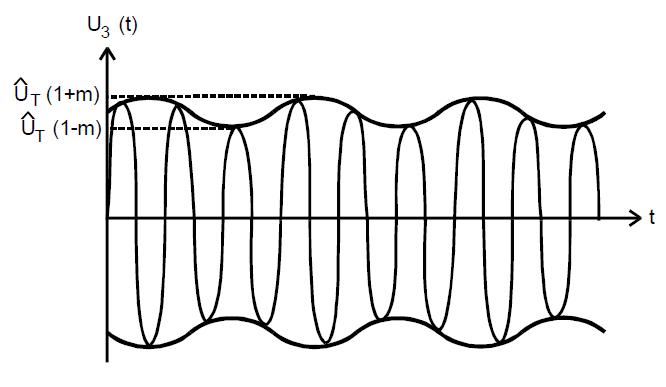
\includegraphics[width=10cm]{images/zeitabhaengigkeit_momentanspannung.png}
\caption{Text}
\label{fig:zeitabhaengigkeit_momentanspannung}
\end{figure}
In Gleichung \ref{eq:amplitudederamplitudenmoduliertenschwingungbesser} ist ersichtlich, dass das Signal bei $\omega_\text{T}$ keinerlei Informationen besitzt, da sie unabhängig von $\hat{U}_\text{M}$ ist. Es wird auch als Trägerabstrahlung bezeichnet und stellt in der Praxis nur einen unnötigen Energieverbrauch da und wird deswegen vermieden.\\
Es kann außerdem Energie gespart werden, indem eines der beiden Bänder durch ein Bandfilter unterdrückt wird. Dies wird auch Einseitenbandmodulation genannt. Es ist möglich, da die beiden Bänder die selbe Information enthalten.
\begin{figure}[H]
\centering 
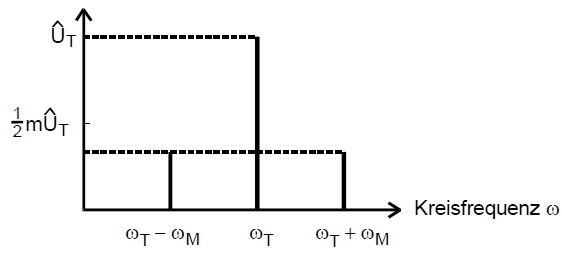
\includegraphics[width=10cm]{images/frequenzsprektum_amplitudenmodulierten.png}
\caption{Text}
\label{fig:frequenzsprektum_amplitudenmodulierten}
\end{figure}
Die Amplitudenmodulation besitzt jedoch eine geringe Störsicherheit und Verzerrungsfreiheit.
\subsection{Frequenzmodulation} 




\section{Durchführung}

\section{Auswertung}

\subsection{Amplitudenmodulation mit Ringmodulator}
Mit einem Ringmodulator wird ein amplitudenmoduliertes SignaL mit Trägerunterdrückung erzeugt. Freequenzen f und Amplituden U von Träger- und Modulationssignal lauten:
\begin{enumerate}
	\item Trägersignal
	\item Modulationssignal 
\end{enumerate}
\subsection{Amplitudendemodulation mit Ringmodulator}

\subsection{Amplitudenmodulation mit Diode}

\subsection{Amplitudendemodulation mit Diode}

\subsection{Frequenzmodulation}

\subsection{Frequenzdemodulation}

\section{Diskussion}

\section{Quellen}

\end{document}